\subsection{Competition results}
The competition took place on two dates (15th and 17th of September) and each team had to play three times against all other teams. Each simulation consisted of a of 400 steps and the team with the highest score at the end got three points for a victory. The team "MaKo" scored second with a total of 18 points. The winner 2014 was, for three times in a row now, the team from the USFC. The overall result looks like the following:
\begin{figure}[h]
	\centering
	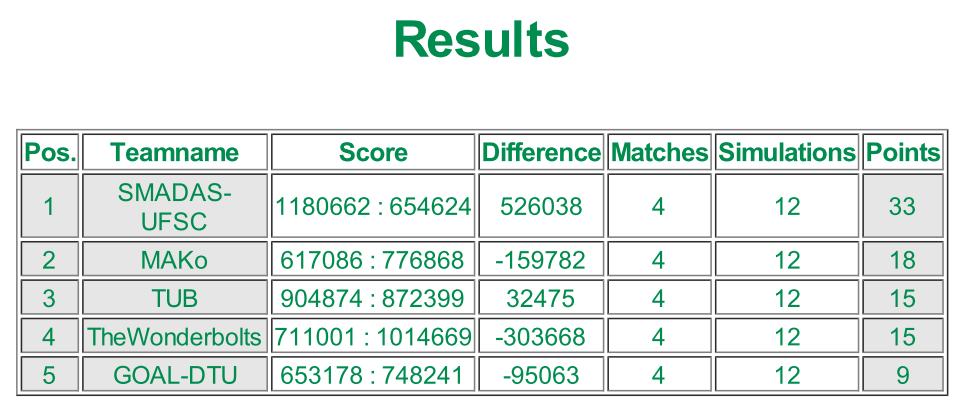
\includegraphics[width=300px]{Result.png}
	\caption{MAPC 2014 result}
	\label{dis:result}
\end{figure}
Statistics of all the individual games can be found in the appendix.[reference here!!!!] 

Team "MaKo" lost every second game against each opponent due to the fact that for some reason the repairer agents weren't able to repair. The reason behind this was not obvious to the team. A strategy that worked out well, was the approach to upgrade the visibility range and the strength of one saboteur agent significantly. In all matches the it was able to disable enemy agents many times and therefore disturb zones and keep the enemy repairers busy, which kept them away from building zones. 
\subsection{Lessons learned}
None of the "MaKo" team member had experience with Jason as a programming language before the research lab. The first thing that causes problems was that Jason was quite slow, especially when it comes to communication between agents. Since agents most times needed some information from others and could not continue with their reasoning until this information was given, communication was a extreme bottleneck. Extreme delay was observed when the group tried to exchange information about the graph. The first approach was to communicate everything that an agent perceives, while exploring the graph, to every other agent. The reason behind this was to have every agent store the full knowledge about the until then explored (sub-)graph. This course of action was quickly discarded, because agents were not able to do actions while processing all the incoming messages. The next attempt to reduce communication was to implement a so called "cartographer" agent. The purpose of this agent was to have an additionally agent in the background that gathers all the information about the map that all 28 agents perceive. With that cartographer agent the amount of communication was reduced and agents could act like intended, because now they just sent their percepts to the cartographer agent and they had not to deal with incoming messages of the other 27 agents. The drawback of this approach revealed when it came to querying the cartographer agent for information, for instance when an agent wanted to know if a vertex was already surveyed or how he could reach given vertex. Like it was noticed before, processing the received messages is quite slow and so it happened that the cartographer agent was not able to handle messages in time. It occurred that agents asked about some specific vertex which the cartographer agent should have known about (because some other agent already informed him about that particular vertex) and they got no answer due to the fact that the cartographer agent hadn't processed the message yet. That's why this approach was also discarded. The next idea, which worked in the end, was to use a Java object, the so called "map agent", for the purpose of storing and processing graph information. Internal actions were used to obtain the required information about the graph. For instance the internal action "getBestHopToVertex" calculates the shortest path and returns, for a given target node, the next vertex where the agent has to go to. 